\documentclass[14 pt]{extarticle}

	\usepackage[frenchb]{babel}
	\usepackage[utf8]{inputenc}  
	\usepackage[T1]{fontenc}
	\usepackage{amssymb}
	\usepackage[mathscr]{euscript}
	\usepackage{stmaryrd}
	\usepackage{amsmath}
	\usepackage{tikz}
	\usepackage[all,cmtip]{xy}
	\usepackage{amsthm}
	\usepackage{varioref}
	\usepackage{geometry}
	\geometry{a4paper}
	\usepackage{lmodern}
	\usepackage{hyperref}
	\usepackage{array}
	 \usepackage{fancyhdr}
\renewcommand{\theenumi}{\alph{enumi})}
	\pagestyle{fancy}
	\theoremstyle{plain}
	\fancyfoot[C]{} 
	\fancyhead[L]{Périmètres}
	\fancyhead[R]{5 mars 2024}\geometry{
 a4paper,
 total={170mm,257mm},
 left=20mm,
 top=20mm,
 }
	
	
	\title{Interrogation chapitre 6}
	\date{}
	\begin{document}

\begin{center}{\Large Interrogation}\\ 
 \end{center}
 \subsection*{Exercice 1}
 Sur votre copie, \textbf{posez} et effectuez les calculs suivants : 
 \begin{enumerate}
 \item $0, 012 -0, 0012$ %2
 \item $98,12 + 23, 78$
 \item $1h 10 min 12 s + 50 min 54 s$
 \item $1h 10 min 12 s - 50 min 54 s$
 \end{enumerate}
 
 
 \subsection*{Exercice 2}
 
 Donnez le périmètre des figures suivantes : 
 \begin{enumerate}
 \item Un carré de côté $3$ cm.
 \item 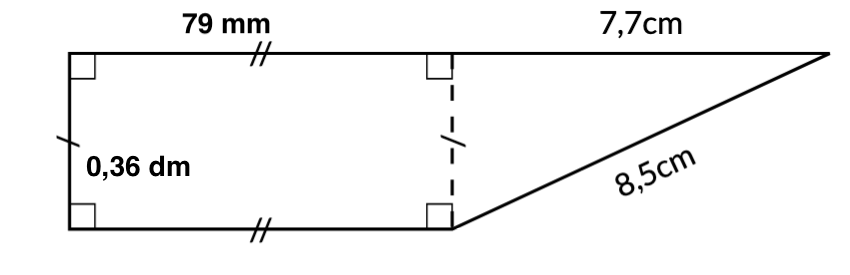
\includegraphics[scale=1]{Exo4a}
 \item 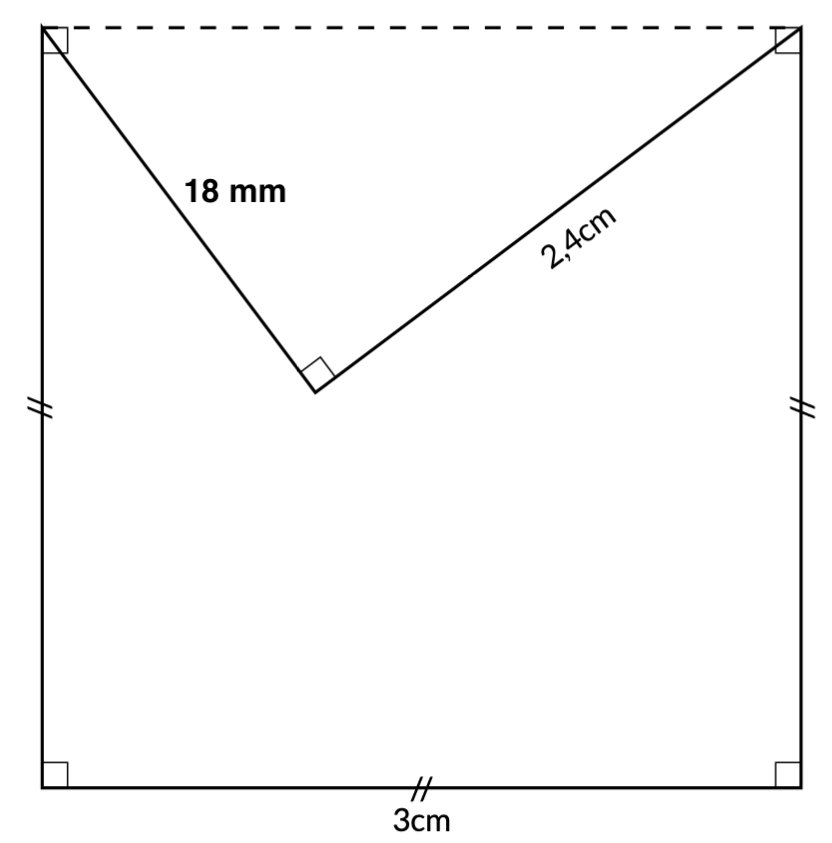
\includegraphics[scale=.5]{Exo4b}
 \item Un hexagone régulier dont les côtés mesurent $3$ cm. 
 \end{enumerate}
 
 \subsection*{Exercice 3}
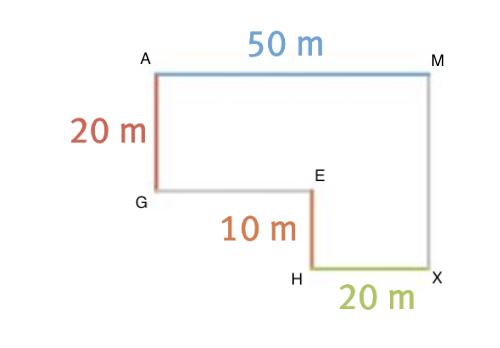
\includegraphics[scale=1]{Exo3}

\begin{enumerate}
\item Combien de côtés a cette figure ? 
\item Comment appelle-t-on un polygone avec ce nombre de côtés ? 
\item Nommer le polygone en utilisant les lettres de la figure. Combien y aurait-il de noms possibles ? 
\item On veut enclore un potager dont la forme est donnée par la figure ci-dessus. Calculez la longueur de clôture nécessaire. 
\item Le fermier, situé au point E, veut aller au point M sans rentrer dans le potager. Quelle distance doit-il parcourir ? (il faut donner la plus courte)
\end{enumerate}
 
 
 
 
 	\end{document}
